
%% bare_jrnl.tex
%% V1.4b
%% 2015/08/26
%% by Michael Shell
%% see http://www.michaelshell.org/ 
%% for current contact information.
%%
%% This is a skeleton file demonstrating the use of IEEEtran.cls
%% (requires IEEEtran.cls version 1.8b or later) with an IEEE
%% journal paper.
%%
%% Support sites:
%% http://www.michaelshell.org/tex/ieeetran/
%% http://www.ctan.org/pkg/ieeetran
%% and
%% http://www.ieee.org/

%%*************************************************************************
%% Legal Notice:
%% This code is offered as-is without any warranty either expressed or
%% implied; without even the implied warranty of MERCHANTABILITY or
%% FITNESS FOR A PARTICULAR PURPOSE! 
%% User assumes all risk.
%% In no event shall the IEEE or any contributor to this code be liable for
%% any damages or losses, including, but not limited to, incidental,
%% consequential, or any other damages, resulting from the use or misuse
%% of any information contained here.
%%
%% All comments are the opinions of their respective authors and are not
%% necessarily endorsed by the IEEE.
%%
%% This work is distributed under the LaTeX Project Public License (LPPL)
%% ( http://www.latex-project.org/ ) version 1.3, and may be freely used,
%% distributed and modified. A copy of the LPPL, version 1.3, is included
%% in the base LaTeX documentation of all distributions of LaTeX released
%% 2003/12/01 or later.
%% Retain all contribution notices and credits.
%% ** Modified files should be clearly indicated as such, including  **
%% ** renaming them and changing author support contact information. **
%%*************************************************************************


% *** Authors should verify (and, if needed, correct) their LaTeX system  ***
% *** with the testflow diagnostic prior to trusting their LaTeX platform ***
% *** with production work. The IEEE's font choices and paper sizes can   ***
% *** trigger bugs that do not appear when using other class files.       ***                          ***
% The testflow support page is at:
% http://www.michaelshell.org/tex/testflow/



%\documentclass[journal,twocolumn]{IEEEtran}
\documentclass[12pt,journal,onecolumn]{IEEEtran}
%
% If IEEEtran.cls has not been installed into the LaTeX system files,
% manually specify the path to it like:
% \documentclass[journal]{../sty/IEEEtran}





% Some very useful LaTeX packages include:
% (uncomment the ones you want to load)


% *** MISC UTILITY PACKAGES ***
%
%\usepackage{ifpdf}
% Heiko Oberdiek's ifpdf.sty is very useful if you need conditional
% compilation based on whether the output is pdf or dvi.
% usage:
% \ifpdf
%   % pdf code
% \else
%   % dvi code
% \fi
% The latest version of ifpdf.sty can be obtained from:
% http://www.ctan.org/pkg/ifpdf
% Also, note that IEEEtran.cls V1.7 and later provides a builtin
% \ifCLASSINFOpdf conditional that works the same way.
% When switching from latex to pdflatex and vice-versa, the compiler may
% have to be run twice to clear warning/error messages.






% *** CITATION PACKAGES ***
%
%\usepackage{cite}
% cite.sty was written by Donald Arseneau
% V1.6 and later of IEEEtran pre-defines the format of the cite.sty package
% \cite{} output to follow that of the IEEE. Loading the cite package will
% result in citation numbers being automatically sorted and properly
% "compressed/ranged". e.g., [1], [9], [2], [7], [5], [6] without using
% cite.sty will become [1], [2], [5]--[7], [9] using cite.sty. cite.sty's
% \cite will automatically add leading space, if needed. Use cite.sty's
% noadjust option (cite.sty V3.8 and later) if you want to turn this off
% such as if a citation ever needs to be enclosed in parenthesis.
% cite.sty is already installed on most LaTeX systems. Be sure and use
% version 5.0 (2009-03-20) and later if using hyperref.sty.
% The latest version can be obtained at:
% http://www.ctan.org/pkg/cite
% The documentation is contained in the cite.sty file itself.






% *** GRAPHICS RELATED PACKAGES ***
%
\ifCLASSINFOpdf
  % \usepackage[pdftex]{graphicx}
  % declare the path(s) where your graphic files are
  % \graphicspath{{../pdf/}{../jpeg/}}
  % and their extensions so you won't have to specify these with
  % every instance of \includegraphics
  % \DeclareGraphicsExtensions{.pdf,.jpeg,.png}
\else
  % or other class option (dvipsone, dvipdf, if not using dvips). graphicx
  % will default to the driver specified in the system graphics.cfg if no
  % driver is specified.
  % \usepackage[dvips]{graphicx}
  % declare the path(s) where your graphic files are
  % \graphicspath{{../eps/}}
  % and their extensions so you won't have to specify these with
  % every instance of \includegraphics
  % \DeclareGraphicsExtensions{.eps}
\fi
% graphicx was written by David Carlisle and Sebastian Rahtz. It is
% required if you want graphics, photos, etc. graphicx.sty is already
% installed on most LaTeX systems. The latest version and documentation
% can be obtained at: 
% http://www.ctan.org/pkg/graphicx
% Another good source of documentation is "Using Imported Graphics in
% LaTeX2e" by Keith Reckdahl which can be found at:
% http://www.ctan.org/pkg/epslatex
%
% latex, and pdflatex in dvi mode, support graphics in encapsulated
% postscript (.eps) format. pdflatex in pdf mode supports graphics
% in .pdf, .jpeg, .png and .mps (metapost) formats. Users should ensure
% that all non-photo figures use a vector format (.eps, .pdf, .mps) and
% not a bitmapped formats (.jpeg, .png). The IEEE frowns on bitmapped formats
% which can result in "jaggedy"/blurry rendering of lines and letters as
% well as large increases in file sizes.
%
% You can find documentation about the pdfTeX application at:
% http://www.tug.org/applications/pdftex





% *** MATH PACKAGES ***
%
%\usepackage{amsmath}
% A popular package from the American Mathematical Society that provides
% many useful and powerful commands for dealing with mathematics.
%
% Note that the amsmath package sets \interdisplaylinepenalty to 10000
% thus preventing page breaks from occurring within multiline equations. Use:
%\interdisplaylinepenalty=2500
% after loading amsmath to restore such page breaks as IEEEtran.cls normally
% does. amsmath.sty is already installed on most LaTeX systems. The latest
% version and documentation can be obtained at:
% http://www.ctan.org/pkg/amsmath





% *** SPECIALIZED LIST PACKAGES ***
%
%\usepackage{algorithmic}
% algorithmic.sty was written by Peter Williams and Rogerio Brito.
% This package provides an algorithmic environment fo describing algorithms.
% You can use the algorithmic environment in-text or within a figure
% environment to provide for a floating algorithm. Do NOT use the algorithm
% floating environment provided by algorithm.sty (by the same authors) or
% algorithm2e.sty (by Christophe Fiorio) as the IEEE does not use dedicated
% algorithm float types and packages that provide these will not provide
% correct IEEE style captions. The latest version and documentation of
% algorithmic.sty can be obtained at:
% http://www.ctan.org/pkg/algorithms
% Also of interest may be the (relatively newer and more customizable)
% algorithmicx.sty package by Szasz Janos:
% http://www.ctan.org/pkg/algorithmicx




% *** ALIGNMENT PACKAGES ***
%
%\usepackage{array}
% Frank Mittelbach's and David Carlisle's array.sty patches and improves
% the standard LaTeX2e array and tabular environments to provide better
% appearance and additional user controls. As the default LaTeX2e table
% generation code is lacking to the point of almost being broken with
% respect to the quality of the end results, all users are strongly
% advised to use an enhanced (at the very least that provided by array.sty)
% set of table tools. array.sty is already installed on most systems. The
% latest version and documentation can be obtained at:
% http://www.ctan.org/pkg/array


% IEEEtran contains the IEEEeqnarray family of commands that can be used to
% generate multiline equations as well as matrices, tables, etc., of high
% quality.




% *** SUBFIGURE PACKAGES ***
%\ifCLASSOPTIONcompsoc
%  \usepackage[caption=false,font=normalsize,labelfont=sf,textfont=sf]{subfig}
%\else
%  \usepackage[caption=false,font=footnotesize]{subfig}
%\fi
% subfig.sty, written by Steven Douglas Cochran, is the modern replacement
% for subfigure.sty, the latter of which is no longer maintained and is
% incompatible with some LaTeX packages including fixltx2e. However,
% subfig.sty requires and automatically loads Axel Sommerfeldt's caption.sty
% which will override IEEEtran.cls' handling of captions and this will result
% in non-IEEE style figure/table captions. To prevent this problem, be sure
% and invoke subfig.sty's "caption=false" package option (available since
% subfig.sty version 1.3, 2005/06/28) as this is will preserve IEEEtran.cls
% handling of captions.
% Note that the Computer Society format requires a larger sans serif font
% than the serif footnote size font used in traditional IEEE formatting
% and thus the need to invoke different subfig.sty package options depending
% on whether compsoc mode has been enabled.
%
% The latest version and documentation of subfig.sty can be obtained at:
% http://www.ctan.org/pkg/subfig




% *** FLOAT PACKAGES ***
%
%\usepackage{fixltx2e}
% fixltx2e, the successor to the earlier fix2col.sty, was written by
% Frank Mittelbach and David Carlisle. This package corrects a few problems
% in the LaTeX2e kernel, the most notable of which is that in current
% LaTeX2e releases, the ordering of single and double column floats is not
% guaranteed to be preserved. Thus, an unpatched LaTeX2e can allow a
% single column figure to be placed prior to an earlier double column
% figure.
% Be aware that LaTeX2e kernels dated 2015 and later have fixltx2e.sty's
% corrections already built into the system in which case a warning will
% be issued if an attempt is made to load fixltx2e.sty as it is no longer
% needed.
% The latest version and documentation can be found at:
% http://www.ctan.org/pkg/fixltx2e


%\usepackage{stfloats}
% stfloats.sty was written by Sigitas Tolusis. This package gives LaTeX2e
% the ability to do double column floats at the bottom of the page as well
% as the top. (e.g., "\begin{figure*}[!b]" is not normally possible in
% LaTeX2e). It also provides a command:
%\fnbelowfloat
% to enable the placement of footnotes below bottom floats (the standard
% LaTeX2e kernel puts them above bottom floats). This is an invasive package
% which rewrites many portions of the LaTeX2e float routines. It may not work
% with other packages that modify the LaTeX2e float routines. The latest
% version and documentation can be obtained at:
% http://www.ctan.org/pkg/stfloats
% Do not use the stfloats baselinefloat ability as the IEEE does not allow
% \baselineskip to stretch. Authors submitting work to the IEEE should note
% that the IEEE rarely uses double column equations and that authors should try
% to avoid such use. Do not be tempted to use the cuted.sty or midfloat.sty
% packages (also by Sigitas Tolusis) as the IEEE does not format its papers in
% such ways.
% Do not attempt to use stfloats with fixltx2e as they are incompatible.
% Instead, use Morten Hogholm'a dblfloatfix which combines the features
% of both fixltx2e and stfloats:
%
% \usepackage{dblfloatfix}
% The latest version can be found at:
% http://www.ctan.org/pkg/dblfloatfix




%\ifCLASSOPTIONcaptionsoff
%  \usepackage[nomarkers]{endfloat}
% \let\MYoriglatexcaption\caption
% \renewcommand{\caption}[2][\relax]{\MYoriglatexcaption[#2]{#2}}
%\fi
% endfloat.sty was written by James Darrell McCauley, Jeff Goldberg and 
% Axel Sommerfeldt. This package may be useful when used in conjunction with 
% IEEEtran.cls'  captionsoff option. Some IEEE journals/societies require that
% submissions have lists of figures/tables at the end of the paper and that
% figures/tables without any captions are placed on a page by themselves at
% the end of the document. If needed, the draftcls IEEEtran class option or
% \CLASSINPUTbaselinestretch interface can be used to increase the line
% spacing as well. Be sure and use the nomarkers option of endfloat to
% prevent endfloat from "marking" where the figures would have been placed
% in the text. The two hack lines of code above are a slight modification of
% that suggested by in the endfloat docs (section 8.4.1) to ensure that
% the full captions always appear in the list of figures/tables - even if
% the user used the short optional argument of \caption[]{}.
% IEEE papers do not typically make use of \caption[]'s optional argument,
% so this should not be an issue. A similar trick can be used to disable
% captions of packages such as subfig.sty that lack options to turn off
% the subcaptions:
% For subfig.sty:
% \let\MYorigsubfloat\subfloat
% \renewcommand{\subfloat}[2][\relax]{\MYorigsubfloat[]{#2}}
% However, the above trick will not work if both optional arguments of
% the \subfloat command are used. Furthermore, there needs to be a
% description of each subfigure *somewhere* and endfloat does not add
% subfigure captions to its list of figures. Thus, the best approach is to
% avoid the use of subfigure captions (many IEEE journals avoid them anyway)
% and instead reference/explain all the subfigures within the main caption.
% The latest version of endfloat.sty and its documentation can obtained at:
% http://www.ctan.org/pkg/endfloat
%
% The IEEEtran \ifCLASSOPTIONcaptionsoff conditional can also be used
% later in the document, say, to conditionally put the References on a 
% page by themselves.




% *** PDF, URL AND HYPERLINK PACKAGES ***
%
%\usepackage{url}
% url.sty was written by Donald Arseneau. It provides better support for
% handling and breaking URLs. url.sty is already installed on most LaTeX
% systems. The latest version and documentation can be obtained at:
% http://www.ctan.org/pkg/url
% Basically, \url{my_url_here}.




% *** Do not adjust lengths that control margins, column widths, etc. ***
% *** Do not use packages that alter fonts (such as pslatex).         ***
% There should be no need to do such things with IEEEtran.cls V1.6 and later.
% (Unless specifically asked to do so by the journal or conference you plan
% to submit to, of course. )


% correct bad hyphenation here
\usepackage{amsmath}
\usepackage{amssymb}
\usepackage{float}
\usepackage{setspace}
\usepackage{lineno}
\usepackage{graphicx}
\usepackage{xr}
%\usepackage{hyperref}


\hyphenation{op-tical net-works semi-conduc-tor}
%\externaldocument{figs}
\graphicspath{{./figures/}}
\doublespacing
\linenumbers


\begin{document}

%
% paper title
% Titles are generally capitalized except for words such as a, an, and, as,
% at, but, by, for, in, nor, of, on, or, the, to and up, which are usually
% not capitalized unless they are the first or last word of the title.
% Linebreaks \\ can be used within to get better formatting as desired.
% Do not put math or special symbols in the title.
\title{Performance of a passive acoustic \\ linear array in a tidal channel}
%
%
% author names and IEEE memberships
% note positions of commas and nonbreaking spaces ( ~ ) LaTeX will not break
% a structure at a ~ so this keeps an author's name from being broken across
% two lines.
% use \thanks{} to gain access to the first footnote area
% a separate \thanks must be used for each paragraph as LaTeX2e's \thanks
% was not built to handle multiple paragraphs
%

\author{Matthew~F.~Auvinen, 
        David~R.~Barclay % <-this % stops a space
\thanks{Dr. David Barclay is an assistant professor in the Department of Oceanography, Dalhousie University. Matthew Auvinen holds a B.Sc. (Hons) from the Department of Oceanography, Dalhousie University, Halifax, NS (email: matthewauvinen@gmail.com; dbarclay@dal.ca).} % <-this % stops a space
\thanks{Manuscript received June 26, 2017; revised MONTH XX, 201X. This work was supported by the Natural Sciences and Engineering Research Council of Canada, GeoSpectrum Technologies, and Black Rock Tidal Power.}}% <-this % stops a space




% note the % following the last \IEEEmembership and also \thanks - 
% these prevent an unwanted space from occurring between the last author name
% and the end of the author line. i.e., if you had this:
% 
% \author{....lastname \thanks{...} \thanks{...} }
%                     ^------------^------------^----Do not want these spaces!
%
% a space would be appended to the last name and could cause every name on that
% line to be shifted left slightly. This is one of those "LaTeX things". For
% instance, "\textbf{A} \textbf{B}" will typeset as "A B" not "AB". To get
% "AB" then you have to do: "\textbf{A}\textbf{B}"
% \thanks is no different in this regard, so shield the last } of each \thanks
% that ends a line with a % and do not let a space in before the next \thanks.
% Spaces after \IEEEmembership other than the last one are OK (and needed) as
% you are supposed to have spaces between the names. For what it is worth,
% this is a minor point as most people would not even notice if the said evil
% space somehow managed to creep in.



% The paper headers
\markboth{IEEE JOURNAL OF OCEANIC ENGINEERING,~Vol.~XX, No.~XX, MONTH~201X}%
{Auvinen and Barclay: Tidal channel array performance}
% The only time the second header will appear is for the odd numbered pages
% after the title page when using the twoside option.
% 
% *** Note that you probably will NOT want to include the author's ***
% *** name in the headers of peer review papers.                   ***
% You can use \ifCLASSOPTIONpeerreview for conditional compilation here if
% you desire.




% If you want to put a publisher's ID mark on the page you can do it like
% this:
%\IEEEpubid{0000--0000/00\$00.00~\copyright~2015 IEEE}
% Remember, if you use this you must call \IEEEpubidadjcol in the second
% column for its text to clear the IEEEpubid mark.



% use for special paper notices
%\IEEEspecialpapernotice{(Invited Paper)}




% make the title area
\maketitle

\begin{abstract}
Baseline ambient sound level assessment is important in quantifying anthropogenic noise contributions. Static acoustic sensing in high-flow conditions is complicated by pseudo-sound, or flow noise, caused by turbulent flow on the surface of a hydrophone. Signal processing methods are used to identify and suppress flow noise at low frequencies ($<$ 500 Hz) in data collected on a four-element horizontal hydrophone array in Minas Passage, a tidal channel in the Bay of Fundy, in October 2016. Spectral slope analysis is used to identify the frequencies at which the flow noise and ambient noise contributions to the recorded signal are equal. The maximum frequencies at which flow noise is observed is determined using analysis of the spatial coherence.  The array's performance in the Minas Passage is quantified by an empirical relationship between flow speed and the spectral critical frequencies of the coherent output from the linear array. Coherent averaging (broadside beamforming) is demonstrated as a potential flow noise suppression technique, improving low-frequency passive acoustic monitoring in a high-energy tidal channel. 
\end{abstract}


\begin{IEEEkeywords}
Flow noise, ambient noise, array processing, tidal channel, and passive acoustic monitoring.
\end{IEEEkeywords}






% For peer review papers, you can put extra information on the cover
% page as needed:
% \ifCLASSOPTIONpeerreview
% \begin{center} \bfseries EDICS Category: 3-BBND \end{center}
% \fi
%
% For peerreview papers, this IEEEtran command inserts a page break and
% creates the second title. It will be ignored for other modes.
\IEEEpeerreviewmaketitle



\section{Introduction}
\label{I}
% The very first letter is a 2 line initial drop letter followed
% by the rest of the first word in caps.
% 
% form to use if the first word consists of a single letter:
% \IEEEPARstart{A}{demo} file is ....
% 
% form to use if you need the single drop letter followed by
% normal text (unknown if ever used by the IEEE):
% \IEEEPARstart{A}{}demo file is ....
% 
% Some journals put the first two words in caps:
% \IEEEPARstart{T}{his demo} file is ....
% 
% Here we have the typical use of a "T" for an initial drop letter
% and "HIS" in caps to complete the first word.
\IEEEPARstart{T}{idal} power utilities are currently leasing seafloor space within the Minas Passage in the Bay of Fundy with hopes of converting the energy of the region's tidal currents into electricity, a trend that has been supported by favorable projections of the Passage's tidal energy capacity \cite{karsten}. It is important that these companies follow sustainable industry practices as the sector grows \cite{yang}. This includes the consideration of industry knowledge gaps, many of which are a consequence of the sector's immaturity \cite{inger}. The uncertainty surrounding the ecological and environmental implications of tidal turbine infrastructure is a particularly important knowledge gap \cite{polagye} and has qualified some opposition to turbine projects. 

One of the main environmental concerns surrounding tidal turbine projects is the threat of physical contact and collision \cite{dadswell} \cite{redden}. The potential of this risk is largely due to uncertainty \cite{copping}. Indeed, the behavioural response of fish and marine mammals to the physical presence of tidal turbines is difficult to monitor and the relationship between tidal turbine infrastructure and local ecosystems is not fully understood. There is evidence that indicates seals actively avoid tidal turbines \cite{hastie}, suggesting that some marine mammals would not suffer from turbine strikes. However, this has not been tested with physical turbines. The uncertainty of other physical threats such as habitat alteration, interference with migrations, and disruption of sediment adds to the perceived risks associated with tidal turbines \cite{polagye}. 

There are also acoustical concerns surrounding tidal energy. Turbines could become an important source of ambient noise in tidal channels through cavitation and mechanical noise \cite{wang}. Turbine anthropophony could affect animal navigation, communication, and predator-prey detections \cite{lombardi}. In some cases the sound generated by tidal turbines could even lead to physical harm \cite{copping}. While there is currently no evidence of turbine operational noise affecting marine animals, there may be risks associated with the noise emitted during the installation of tidal turbines, especially if pile driving is involved \cite{polagye}. %risks associated with turbine installation are uncertain \cite{7914}. %Many of these risks are uncertain and difficult to investigate \cite{7914}.  and marine life cycles \cite{pine}. Moreover, turbine-generated sound could be damaging to fish tissue \cite{halvorsen}. If substantive, these effects would threaten near-field and far-field ecosystem health, stressing the need for rigorous environmental impact assessments in the tidal power sector. 

These environmental risks emphasize the need for baseline ambient noise measurements in the Minas Passage, against which turbine noise pollution can be measured. However, the utility of ambient sensing is limited by pseudo-sound, or flow noise, generated on the surface of a hydrophone in turbulent water. The masking effects of flow noise can complicate source identification and background noise assessment in high-flow settings, such as tidal channels.

Similar to turbulent flowing air \cite{light}, flowing water in a high Reynolds number regime generates pressure fluctuations on the surface of a hydrophone. These pressure fluctuations produce flow noise which is irregular, uncorrelated, and random. Local pressure fluctuations on the surface of a hydrophone represent near-field turbulence \cite{strasberg}. Free-drifting hydrophones moving with the mean water flow will experience little signal contamination, as it is the relative flow of water over a hydrophone's surface that leads to flow noise.  

%Turbulent flows occupy a wide range of frequencies and wavenumber domains, with broad spatial and temporal variability. The advective nonlinearity %and sensitivity 
%of turbulent flows makes them unpredictable in space and time, and contributes to their complex nature \cite{van}. As such, it is difficult to reliably model flow noise. 
Flow noise follows a spectral slope of $f^{-5/3}$ at low frequencies, behaviour that is analogous to Kolmogorov's turbulence theory. This flow noise is not to be confused with wind-generated noise that produces $f^{-5/3}$ spectral slopes at higher frequencies \cite{knud}. Bassett et al. \cite{bassett} identifies $f^{-5/3}$ flow noise below 20 Hz and also describes steepened spectral slopes, $f^{-m}$, between 20 and 200 Hz. Lombardi \cite{lombardi} identifies the same steepened spectral slopes in measurements from the Grand Passage tidal channel. The flow noise that produces $f^{-m}$ is a result of small-scale turbulence being averaged out across the surface of the hydrophones, which dampens (or reduces) measurements.

Flow noise presents a unique challenge for passive acoustic monitoring (PAM): a hydrophone in a high-flow setting will record both propagating sound and pseudo-sound. This suggests that models should distinguish between the two sound sources. While flow noise and ambient noise are inseparable, the masking effects of flow noise can be addressed by exploiting its uncorrelated nature. This has been done using ambient noise coherence, cross-correlation, and covariance \cite{barclaywind} \cite{chung} \cite{buck2}.  %We adapt this application of coherence to identify and suppress flow noise across a four-element array in a tidal channel.  

Successful suppression of flow noise could benefit PAM systems in relatively energetic environments.
The objectives of the present research are: 
\begin{enumerate}
\item Use spectral analysis and spatial coherence to identify and characterize flow noise at low frequencies ($<$ 500 Hz).
\item Use coherent averaging (beamforming) to improve the performance of a linear hydrophone array by suppressing flow noise and enhancing the measurement of ambient noise. 
\end{enumerate}

This paper is organized as follows. Section II discusses important field work details, including an experiment description and instrumentation summary. Section III describes all relevant signal processing, with emphasis on spectral analysis, spatial coherence, and beamforming. Section IV presents the signal processing and data analysis results. Section V evaluates the results and identifies areas for future work. Lastly, Section VI summarizes the findings of the study in a series of conclusions.


%%%%%%%%%%%%%%%%%%%%%%%%%%%%%%%%%%%%%%%%%%%%%%%%%%%%%%%%%%%%%%%%%%%%



\section{Field Work}
\label{II}

Field work was completed on October 27, 2016, near the Fundy Ocean Research Center for Energy (FORCE) site in the Minas Passage of the Bay of Fundy. The FORCE site depth ranges between 40 and 60 meters depending on the tide. The deployment period spanned roughly four hours, from 12:00 ADT to 16:00 ADT. This experimental window captured the transition from ebb tide to slack tide. 

Wind speed was measured intermittently throughout the deployment period using a hand-held wind speed gauge. Throughout the observation period wind speed was low and the ocean surface was relatively calm. Tidal data was generated using a WebTide model \cite{webtide}. 

There is a substantial fish population in the Minas Passage \cite{dadswell}, some of which could contribute to the local ambient sound field \cite{wilson}. Pilot whales, dolphins, seals, and other marine mammals that frequent the Minas Passage are another potential source of ambient noise. These animals generate sound through a variety of mechanisms, such as muscle action, stridulation, and vocalization \cite{hilde}. Non-biological sound sources in the Minas Passage include wave action, anthropogenic activity, and bubbles. Proper characterization of the local sound field at the FORCE site would require consideration of these potential sound sources. However, their variability makes source identification challenging. 



\subsection{Experiment}
A linear hydrophone array was streamed behind the \textit{MV Nova Endeavour} (42' x 16'), which was anchored to the seafloor of the Minas Passage while in dead ship. The array was positioned roughly 15 meters below the sea surface using a towfish depressor. The strength of the current kept the array at a relatively constant depth throughout the experiment. Four hydrophones were simultaneously sampled over a four hour period and processed by an analog-to-digital converter (ADC) on board the \textit{MV Nova Endeavour}. The signal cable, which carried both the array and a drogue, was sheathed in a fairing to reduce strum generation and attached to a tow cable (6GA galvanized wire) using cable ties.

A drifting hydrophone (Geospectrum Technologies GuardBuoy) was deployed using a small auxiliary vessel launched from the \textit{MV Nova Endeavour}. The GuardBuoy was suspended 2 meters below the surface using a drifting surface float and isolation system made of a damping mass, a Dacron non-stretch line, and a compliant bungee.  The system isolated the recording hydrophone and instrument package from any surface action, such as the vertical movement of waves, which would otherwise generate mechanical or flow noise.

A total of five GuardBuoy casts were performed by driving the GuardBuoy upstream in a rigid-hulled inflatable boat (RHIB), turning off the RHIB engines, deploying the drifter, floating downstream in the RHIB alongside the drifter, and retrieving the drifter once it had reached 20 meters beyond the array. A separation distance of at least 10 meters was maintained between the drifter and the RHIB while floating downstream. It is important to note that the drifter transects passed over the array. 

These transects were performed over the course of three hours, beginning at 13:00 ADT. The GuardBuoy signals are assumed to be free of flow noise and were used as benchmarks to assess the performance of the array. The turbulent tidal channel is assumed to be well mixed with an isovelocity sound speed profile, minimizing noise field variability over the depth difference between the two systems.



\subsection{Instrumentation}
The linear array is an oil-filled array with a rigid exterior and acoustically transparent outer skin. It contains four sequentially spaced hydrophones with a horizontal configuration along the axis of the array. The array and the hydrophones were constructed by GeoSpectrum Technologies. Each neighbouring hydrophone is separated by a distance $d$ = 17cm. The array hydrophones were set to simultaneously sample at a rate of 96 kHz with an acoustic bandwidth of 48.019 kHz.
The four channels on the array continuously recorded 10 minute WAV files over a 4 hour period. Power spectra were calibrated to dB re 1 $\mu$Pa$^2$/Hz according to frequency-dependent sensitivities supplied by the manufacturer. The GuardBuoy sampled at a rate of 96 kHz with an acoustic bandwidth of 48 kHz, and was equipped with a GPS to record transect geospatial information. The Guard Buoy recorded WAV files in 30 minute segments. Corresponding power spectra were converted to dB re 1 $\mu$Pa$^2$/Hz according to frequency-dependent sensitives supplied by the manufacturer. 




%%%%%%%%%%%%%%%%%%%%%%%%%%%%%%%%%%%%%%%%%%%%%%%%%%%%%%%%%%%%%%%%%%%%



\section{Data Analysis}
\label{III}
Data analysis was performed in MATLAB in several stages. The analysis began with the calculation of the power spectral density (PSD) from the raw WAV files, followed by spectral analysis, spatial coherence analysis, and broadside beamforming. 



\subsection{General Signal Processing}

The output of a hydrophone is defined as
\begin{align}
x_i(t) = \sigma_i(t) + n_i (t) 
\label{output}
\end{align}
where $x_i$ is the recorded time series on each $i$th hydrophone, $\sigma_i$ is the sound field's ambient components, and $n_i$ is the locally generated flow noise. Importantly, $n_i$ and $\sigma_i$ are uncorrelated. 
Furthermore, the inherent randomness of flow noise makes $n_i$ incoherent with  respect to $n_j$. 

The power spectrum, or spectral density, is defined as 

\begin{align}
S_{ii}(\omega) = \frac{\langle X_i(\omega)\cdot X_i^*(\omega) \rangle}{T}
\label{power}
\end{align}
where $X_i$ is the Fourier transform of $x_i$, $\omega$ is angular frequency, * denotes a complex conjugate, $\langle \rangle$ indicates an ensemble average, and $T$ is the observation interval. All Fourier transforms are windowed by a Hann function and the Hann function's effect on the variance has been accounted for. The time series were divided into 34.1 second-long segments, where each segment was further split into 50 contiguous subsegments of 0.682s with no overlap. A $2^{16}$ Fourier transform was applied to each subsegment, from which ensemble averaging produced a power spectral density with a frequency bin width of 1.47 Hz. Coherence is used to quantify the similarity between two signals and is defined as 

\begin{align}
\Gamma_{ij}(\omega) = \frac{S_{ij}(\omega)}{(S_{ii}(\omega) \cdot S_{jj}(\omega))^{\frac{1}{2}}}.
\label{coherence}
\end{align}



\subsection{Power Spectrum Probability Density}

Spectral probability density (SPD) is an analytical technique used to depict the variability of the power spectrum over a period that is much longer than the minimum time required for a stationary measurement of power to be made \cite{merchant}. This form of analysis facilitates the identification of unique events within a series of spectra. The power spectrum probability density (PSPD) is defined as

\begin{align}
\text{PSPD}(f) = H(S_{ii}(f),h)
\label{PSPD_definition}
\end{align}
where PSPD$(f)$ is the power spectrum probability density at frequency $f$, and $H(S(f),h)$ is the histogram of the power spectrum $S_{ii}$ at frequency $f$ with a histogram bin width of $h$  dB re 1 $\mu$Pa$^2$/Hz. By combining PSPD results across frequencies, we generate a PSPD matrix 
\begin{equation}
\begin{bmatrix}
\text{PSPD}(f_1) & \text{PSPD}(f_2) & \text{PSPD}(f_3) & \dots &\text{PSPD}(f_a)
\end{bmatrix}
\label{PSPD_matrix}
\end{equation}
where PSPD$(f_a)$ is the PSPD at the $a$th frequency. 



\subsection{Spectral Critical Frequency}
Lombardi \cite{lombardi} and Bassett et al. \cite{bassett} suggest that there are three distinct spectral slope regions in the low-to-mid-frequency range: spectral slopes of Kolmogorov's $f^{-5/3}$; steepened flow noise spectral slopes, $f^{-m}$, that include the effects of a finite volumed sensor \cite{bassett}; and an ambient noise region that is determined by near-field and far-field ambient sound sources.

The local spectral slope is defined as

\begin{align}
-M = \frac{S_{ii}(2\pi f_a) - S_{ii}(2\pi f_b)}{\log(f_a \cdot f_b^{-1})}
\label{slope}
\end{align}
where $S_{ii}(2\pi f_a)$ is the spectral density on the $i$th sensor at frequency $f_a$ and $S_{ii}(2\pi f_b)$ is the spectral density on the $i$th sensor at frequency $f_b$. The spectral slope in dB/decade is described by \eqref{slope}. 

The transition from the flow noise region of $f^{-m}$ to the ambient noise region is marked by the frequency knee, where the spectral slope begins to shallow. That is, the exit from the flow noise region is marked by a deviation below the slope $f^{-m}$. Here, the spectral critical frequency, $f_c$, is defined as the first frequency at which 

\begin{align}
|M| < |m|
\label{fc}
\end{align}
is true. Both slopes in \eqref{fc} are in dB/decade.



\subsection{Coherence Critical Frequency}
Spatial coherence is calculated for each channel combination using \eqref{coherence}, providing an assessment of signal similarity between elements. Propagating ambient noise is highly correlated across the array. Additionally, propagating noise at wavelengths sufficiently large relative to element spacing produces very high coherence at low frequencies by effectively co-locating sensors. Conversely, flow noise is a source of incoherence, as pseudo-sound is uncorrelated across the linear array (when turbulent scales are smaller than hydrophone separation). Therefore, in the band $f$ $<$ 500 Hz, flow noise is marked by low coherence while ambient noise is marked by high coherence. The transit of this coherence boundary, from flow noise (incoherent) to ambient noise (coherent) provides a metric for describing the extent of flow noise across the array. 

The coherence critical frequency, $f'_c$, is defined as the frequency at which a minimum coherence threshold is crossed due to flow noise masking. To establish this coherence threshold, we assume an isotropic ambient noise field such that the horizontal coherence is given by Buckingham \cite{buck}

\begin{align}
G_{ij}(\omega^\prime) = \frac{\sin (\omega_{ij}^\prime)}{\omega_{ij}^\prime}
\label{theoretical_coherence}
\end{align}
where

\begin{align}
\omega_{ij}^\prime = \frac{2\pi d_{ij}f }{c}.
\label{w}
\end{align}
Here, $d_{ij}$ is the separation distance between the $i$th and $j$th hydrophone and $c$ is the local sound speed. We define $f^\prime_c$ as the first frequency at which 

\begin{align}
|\Gamma_{ij}(\omega^\prime)|\geq  0.9\cdot G_{ij}(\omega^\prime)
\label{crit_coh}
\end{align}
is true. 
We can be confident that any coherence within 10\% of \eqref{theoretical_coherence} is real and significant while any drop below the threshold given by the right hand side of \eqref{crit_coh} is caused by the addition of flow-generated incoherent noise. 
This automated critical frequency detector corresponds to a coherence threshold of $\sim$ 0.9. The use of a more sophisticated noise model such as Cron and Sherman \cite{cron} or Deane et al. \cite{deane} in the place of \eqref{theoretical_coherence} yields a nearly identical threshold.



\subsection{Linear Regression}

Least squared linear regressions between critical frequencies,  $f_c$ and $f'_c$, and flow speed, $u$, are used to identify and characterize the prevalence of flow noise and ambient noise in measurements. 



\subsection{Beamforming }

We use a broadside beamformer to coherently average the channels across the array. Locally generated flow noise and the ambient sound field are inseparable, however we can describe their relative prevalence with the theoretical signal-noise ratio (SNR) where we are defining ambient sound as the signal, and flow noise as the noise. By taking the Fourier transform of \eqref{output} and substituting into \eqref{power}, we find

\begin{align}
S_{ii} &= \frac{\langle (\varsigma_i + N_i)\cdot(\varsigma^*_i + N^*_i) \rangle}{T}
\label{SI}
\end{align}
where $\varsigma_i$ and $N_i$ are the Fourier transforms of $\sigma_i$ and $n_i$, respectively. For clarity, the frequency dependency has been omitted. Since $\varsigma_i$ and $N_i$ are uncorrelated, we can expand \eqref{SI} to arrive at

\begin{align}
S_{ii} &= \frac{\langle \varsigma_i \varsigma^*_i \rangle + \langle N_i N^*_i \rangle}{T}.
\label{ensemble}
\end{align}

Given \eqref{ensemble}, the SNR for a single hydrophone (SNR$_H$) is defined as	

\begin{align}
\text{SNR}_H = \frac{\langle \varsigma_i \varsigma^*_i \rangle}{\langle N_i N^*_i \rangle}
\label{SNR}
\end{align}
where SNR$_H$ = 1 at the critical frequency, $f_c$. Now consider an array of hydrophones indexed by $i$, where the ambient sound field component of the signal on each phone is

\begin{align}
\sigma_{i+1}(t) = \sigma_1(t-\tau_{i}) \quad \quad \text{ } (i>1)
\label{delay}
\end{align}
where 

\begin{align}
\tau_i = \frac{i\cdot d \cos\theta}{c}
\label{tau}
\end{align}
is the acoustic travel time in seconds for plane wave noise arriving on the sensors at the angle $\theta$. Here, $d$ is the nearest neighbour element separation.  Taking the Fourier transform of \eqref{delay} gives 

\begin{align}
\varsigma_i(\omega) = \varsigma_1(\omega) e^{-i \omega \tau_{i}}.
\label{array_power}
\end{align}

The coherent sum of the signals across the array is defined as 

\begin{align}
x_T(t) = \sum_{i = 1}^{l} x_i(t)
\label{xt}
\end{align}
where $x_i(t)$ is the signal recorded on the $i$th element of a linear array $l$ elements long. Since no time delay has been applied to $x_i(t)$, $x_T(t)$ is the equivalent to beamforming broadside to the array. Since the source of interest is ambient noise, the sound field is assumed to be axially symmetric. Thus the horizontal array orientation and beam direction are unimportant, provided an appropriate array gain compensation is applied. 

The Fourier transform of \eqref{xt} is 

\begin{align}
X_T(\omega) = \sum_{i = 1}^{l} X_i(\omega).
\label{XT}
\end{align}
The array power spectral density can be estimated using \eqref{XT} by

\begin{align}
A = \frac{\langle X_T(\omega) \cdot X^*_T(\omega) \rangle}{T}.
\label{A}
\end{align}
Given an array with both ambient noise and flow noise components, \eqref{XT} can be expanded to

\begin{align}
X_T = [ \varsigma_1 + N_1 + \varsigma_2 + N_2 + \dots \varsigma_l + N_l ]
\label{expanded_XT}
\end{align}
which describes the total output of all sensors on an array with $l$ elements. Substituting \eqref{array_power} into \eqref{expanded_XT} gives

\begin{align}
X_T = \varsigma_1 + N_1 + \sum_{i=1}^{l}( \varsigma_1 e^{-i \omega \tau_{i}} + N_{i+1}).
\label{EXTENDED_XT}
\end{align}
Using the Fourier transform of the coherently summed outputs across the array, the power spectral density can be computed by substituting \eqref{EXTENDED_XT} into \eqref{A} yielding

\begin{align}
A =\frac{\langle \varsigma_1\varsigma^*_1 \Big [ l + \sum \limits_{i=1}^{l-1}\frac{1}{2}\Big (l - i \Big )\cos(\omega \tau_{i}) \Big ] + N\cdot N^* \rangle}{T}
\label{A_expanded}
\end{align}
where

\begin{align}
N = \sum_{i}^{l} N_i 
\label{N}
\end{align}
is the coherently summed flow noise. This term can be simplified by assuming the power of the flow noise measured on each individual hydrophone is equal across the array, 

\begin{align}
\langle N_i N^*_i \rangle = \langle N_j N^*_j \rangle 
\label{assume}
\end{align}
and uncorrelated between the sensors,

\begin{align}
\langle N_i N^*_j \rangle = \delta_{ij} \cdot N_1 N^*_1
\label{ASSUME}
\end{align} 
\[
\delta_{ij}=
\begin{cases}
0&\text{if }i\neq j\,\\
1 &\text{if }i=j.
\end{cases}
\]
Then the total power received by the array becomes 

\begin{align}
A = \frac{\langle \varsigma_1\varsigma^*_1 \rangle \Big [ l + \sum \limits_{i=1}^{l-1}\frac{1}{2}\Big (l - i \Big )\cos(\omega \tau_{i}) \Big ] + l\langle N_1 N^*_1 \rangle }{T}.
\label{A_EXPANDED}
\end{align}
Furthermore, if $K$ is defined as

\begin{align}
K =  l + \sum_{i=1}^{l-1}\frac{1}{2}\Big (l - i \Big )\cos(\omega \tau_{i}) 
\label{shortened}
\end{align}
then \eqref{A_EXPANDED} becomes

\begin{align}
A = \frac{K\langle  \varsigma_1 \varsigma^*_1 \rangle  + l\langle N_1 N^*_1 \rangle}{T}
\label{shortened_A}
\end{align}
where \eqref{shortened_A} describes the array spectral density. Here, $SNR_A$ describes the relative strength of the ambient noise and flow noise components of the array output, such that

\begin{align}
\text{SNR}_A = \frac{K  \langle \varsigma_1 \varsigma^*_1 \rangle}{l\langle N_1 N^*_1 \rangle}.
\label{SNR_A}
\end{align}

Comparing \eqref{SNR_A} to the result derived for a single hydrophone, given by \eqref{SNR}, we see that the beamformed array improves the signal-to-noise ratio by a factor of $\frac{K}{l}$. Furthermore, \eqref{SNR_A} suggests that array performance improves with an increasing number of hydrophones, $l$. For an array with 4 elements, at broadside, $\frac{K}{l}$ = $\frac{7}{4}$.



\subsection{Array Gain}
The broadside beamforming analysis applied to the linear array generates artificial spectral density gain. As a result, an array gain formula is applied to the beamformed results to correct the inflated values. The array gain formula presented here is adapted from Cox \cite{cox}, such that

\begin{align}
AG = 10 \log l.
\label{gain}
\end{align}
The array gain correction is performed by subtracting the result of \eqref{gain} from the calculated array power spectral density.
\subsection{Algorithm Assessment}
All channel signals are consolidated into one coherent array output using \eqref{XT} and \eqref{A}. The resulting coherent array signal is compared to signals from the GuardBuoy and a single fixed hydrophone to evaluate the performance of the beamformed array. The algorithm is further tested by comparing the coherent array spectral critical frequencies  to the spectral critical frequencies of a fixed single hydrophone. 

%%%%%%%%%%%%%%%%%%%%%%%%%%%%%%%%%%%%%%%%%%%%%%%%%%%%%%%%%%%%%%%%%%%%
\section{Results}
\label{IV}



\subsection{Spectral Density}

A comparison between spectral density and current speed (Fig. \ref{f:power}) reveals high signal levels in fast flowing water and low signal levels in slow flowing water. The signal power is high below 10 Hz and falls off as the frequency approaches 100 Hz, which indicates that flow noise is prevalent at low frequencies. 

The hydrophone power spectrum contains multiple episodes of mid-frequency noise. These signals are attributed to ship noise generated by passing ships and the small vessel used in the GuardBuoy drifter tests. The abrupt shift in spectral density at 90 minutes is attributed to a reset of the ground between the data acquisition hardware and the array housing. The data collected during this reset have been omitted.

\begin{figure}[!t]
	\begin{center}	
		\includegraphics[width=0.65\textwidth]{figure1.eps} 
	\end{center}
	\caption[Hydrophone power spectra]{
	\label{f:power}
Power spectrum for channel 0 on the array (a). The spectrum is plotted over the deployment period across a range of low-to-mid frequencies. Data sampling errors are marked by E1 and E2 and different mid-frequency noise events, such as ship noise, are marked by E3 - E6. The data from these events has been omitted from the spectral and coherence analyses. The spectrum begins at maximum ebb tide and ends shortly after slack tide, as shown by the current speed time series (b). Power decreases with current  speed over the deployment period. }
\end{figure}

\subsection{Power Spectrum Probability Density}
The PSPD ( Fig. \ref{f:lines}) facilitates the broad-scale assessment of a hydrophone's spectral density over entire deployment periods. The PSPD follows a spectral slope of $f^{-5/3}$ below 10 Hz, behaviour analogous to Kolmogorov's turbulence theory. This spectral slope marks a region of flow noise within the signal. A steepened spectral slope of $f^{-m}$, where $m>\frac{5}{3}$, persists between 40 and 100 Hz, a result of small-scale turbulence when turbulence wavelength $<<$ sensor size. This small-scale turbulence is averaged out over the surface of the hydrophone sensor, dampening the measured signals. The PSPD results show that ambient noise is dominant above 300 Hz, where signal levels are markedly low. Single power spectra are superimposed on the PSPD and suggest that measurements in slow current conditions contain a greater extent of ambient noise relative to those in fast current conditions. 

Early in the deployment (around 10 minutes) electronic noise in the system raised the noise floor to 90 dB $\mu$Pa. While this was quickly remedied on site and has been accounted for in the data, a noise floor persisted around 60 dB $\mu$Pa. 

\begin{figure}[!t]
	\begin{center}
		\includegraphics[width=0.7\textwidth]{figure2.eps} 
	\end{center}
	\caption[Power spectrum probability density]{
	\label{f:lines}
	Fixed single hydrophone power spectrum probability density over the entire deployment period. Turbulent flow noise is prevalent $<$ 10 Hz (where wavelengths $>>$ sensor size), with a spectral slope of $f^{-5/3}$, while turbulence interacting with the hydrophone's finite volume (in the 10 Hz to 100 Hz band) yields a spectral slope of $f^{-m}$. The ambient sound field dominates at frequencies $>$ 300 Hz. Coloured lines represent individual spectra recorded at the time after deployment indicated in the legend.}
\end{figure}


\subsection{Spectral Critical Frequency}
Spectral slopes were calculated between 40 and 100 Hz for each minute of deployment using \eqref{slope}. The linear relationship between spectral slope, $m$, and current speed, $u$, (Fig. \ref{f:slopes}) indicates that signals recorded in decreasing flow are increasingly dampened (steepened slope). The inverse relationship between current speed and spectral slope suggests that signals are less dampened in fast flowing water, a result of larger turbulence scales. The spectral slopes observed between 40 and 100 Hz range from -25 to -60 dB/decade. The correlation coefficient, R, indicates that there is a meaningful correlation between spectral slope and current.
\begin{figure}[!t]
	\begin{center}
		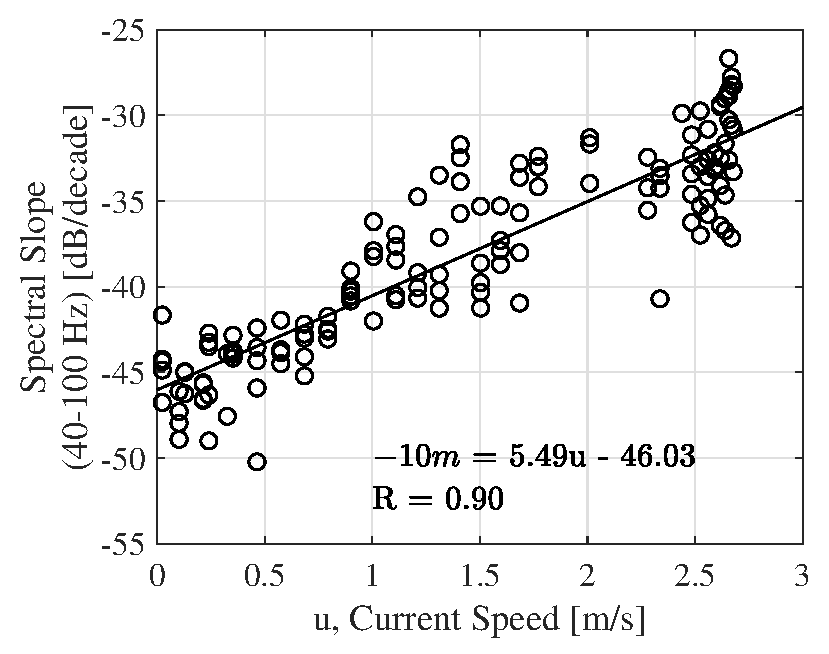
\includegraphics[width=0.7\textwidth]{figure3.eps} 
	\end{center}%
	\caption[Spectral slope current speed dependence]{
	\label{f:slopes}
	Relationship between spectral slope, $m$, and current speed, $u$, between 40 and 100 Hz for channel 0. Spectral slope magnitude increases with decreasing flow. The correlation coefficient, R, is reported. }
\end{figure}


The spectral critical frequency is the frequency at which flow noise and ambient noise are equal in power, and was calculated for each minute of deployment using \eqref{fc}. These critical frequencies were regressed against current speed, as shown in Fig. \ref{f:thresh}. There is a positive correlation between spectral critical frequency and current speed, where fast flow coincides with high spectral critical frequencies. 

The intercepts have not been forced to zero. This is because it is unrealistic to expect that we can completely eliminate flow noise, or low-frequency noise generated by the mechanical systems that comprise the tow body. If this were a moored system with no surface expression, that assumption might be valid, but is not considered here. 
\begin{figure}[!t]
	\begin{center}
		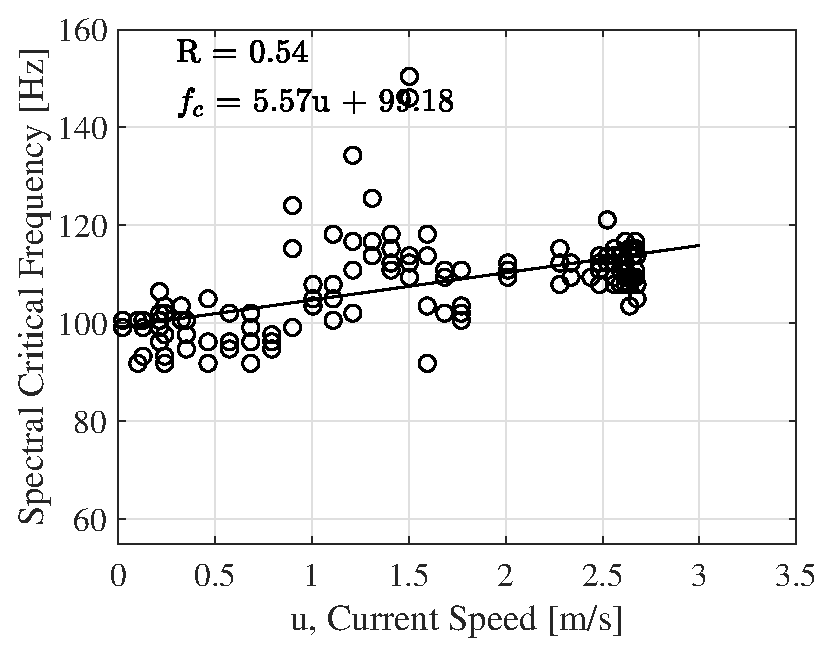
\includegraphics[width=0.7\textwidth]{figure4.eps}
	\end{center}
	\caption[Spectral slope thresholding results]{
	\label{f:thresh}
	Relationship between spectral critical frequency, $f_c$, and current speed, $u$, for channel 0. Spectral critical frequency marks where the flow noise and ambient noise contributions to the recorded signal are equal, and increases with current speed. The correlation coefficient, R, is reported.}
\end{figure}




\subsection{Spatial Coherence}
Spatial coherence is calculated for different hydrophone combinations across the linear array using \eqref{coherence}. The spatial coherence results are presented in magnitude coherence for the entire deployment period (Fig. \ref{f:coherence}). 
\begin{figure}[!t]
	\begin{center}
		\includegraphics[width=0.7\textwidth]{figure5.eps}
	\end{center}
	\caption[Hydrophone spatial coherence]{
	\label{f:coherence}
	Spatial coherence over the experimental period. Magnitude coherence is expected to tend to unity as the fixed hydrophones become relatively co-located. However, uncorrelated flow noise on each phone breaks that relationship. The extent of incoherent flow noise increases with current speed. Channel 0 - 1 (a) and 0 - 3 (b) are shown as examples. Results hold to all other channel combinations.}
\end{figure}
If the wavelength of propagating sound is sufficiently long (frequency sufficiently low) the sensors would become relatively co-located and the coherence would tend to unity. 
However, the results suggest that the low frequency data is overwhelmingly incoherent, since the locally generated flow noise is incoherent from one hydrophone to the next. 

Flow noise is uncorrelated and propagating ambient noise is highly correlated at low frequencies. As a result, low coherence and high coherence are a sign of flow noise and ambient noise, respectively. Therefore, the spatial coherence results are partitioned into two distinct regions: a flow noise region and an ambient noise region. Visual assessment suggests that flow noise is consistently present at low frequencies and can be prominent at higher frequencies (above 600 Hz). The ambient noise region is present between 200 and 600 Hz and contains the same vessel noise identified in Fig. \ref{power}. 



\subsection{Coherence Critical Frequency}
\begin{figure}[!t]
	\begin{center}
		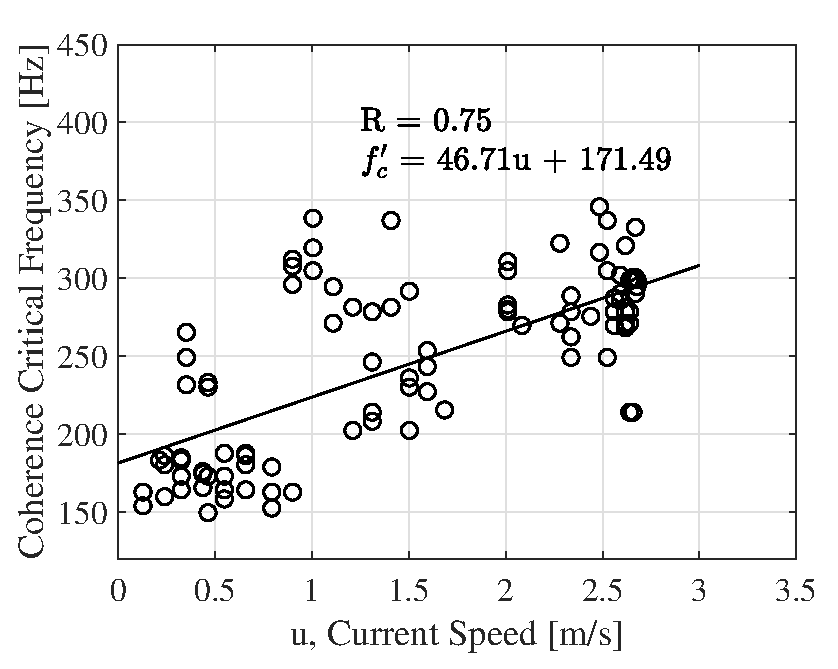
\includegraphics[width=0.7\textwidth]{figure6.eps}
	\end{center}%
	\caption[Spatial coherence thresholding results.]{
	\label{f:c_thresh}
	Relationship between coherence critical frequency, $f^\prime_c$, and current speed, $u$, for channels 0 - 1. Coherence critical frequency is the highest frequency at which flow noise can be detected, and increases with current speed. }
\end{figure}
The coherence critical frequency is the highest frequency at which flow noise can be detected. The coherence critical frequency was calculated for each minute of deployment for each combination of channels, and is used to quantify the relative prevalence of flow noise and ambient noise within a measurement (Fig. \ref{f:c_thresh}). The coherence critical frequency is a more sensitive method of flow noise measurement than the spectral critical frequency, as spatial coherence is used as an indicator of flow noise cessation rather than relative noise contributions. The coherence critical frequency increases with increasing flow speed, a relationship similar to that of the spectral critical frequency. 

It is important to note that the coherence is impacted by any temporary deterministic noises present in the sound field, such as the auxiliary RHIB, mechanical array noise, or noise generated aboard the \emph{MV Nova Endeavour}. In such instances, the automated coherence critical frequency detector fails, and yields an outlier. These outliers have been removed.




\subsection{Beamforming}
The spectral critical frequency of the coherent array output is compared to the fixed single hydrophone spectral and coherence critical frequencies in Fig. \ref{f:array_perform}. 
The standard deviations of the spectral slope and spatial coherence critical frequency regressions were extracted from the averaged fits, while the standard deviation of the coherent array critical frequency regression was calculated from the data during the regression.

The coherence critical frequencies are relatively high, while spectral critical frequencies (both fixed single hydrophone and coherent array) are relatively low. This is attributed to the more sensitive nature of the coherence-based method. Above coherence critical frequencies we can be confident that there is no contamination of the ambient noise field by flow noise. Conversely, the fixed single hydrophone and coherent array spectral critical frequencies show where flow noise and ambient noise have equal power. The coherence and spectral critical frequencies serve as the respective upper and lower bounds of different noise regimes. The coherent array output contains lower critical frequencies than the fixed single hydrophone, indicating that the broadside beamforming approach lessens the extent of flow noise within the measurements. 


Fig. \ref{f:comparison} compares GuardBuoy, fixed single hydrophone, and horizontal coherent array power spectra at 1.5 hours into the experiment. At this time the drifter and array were in close proximity and the current was 2.2 m/s. 
\begin{figure}[!t]
	\begin{center}
		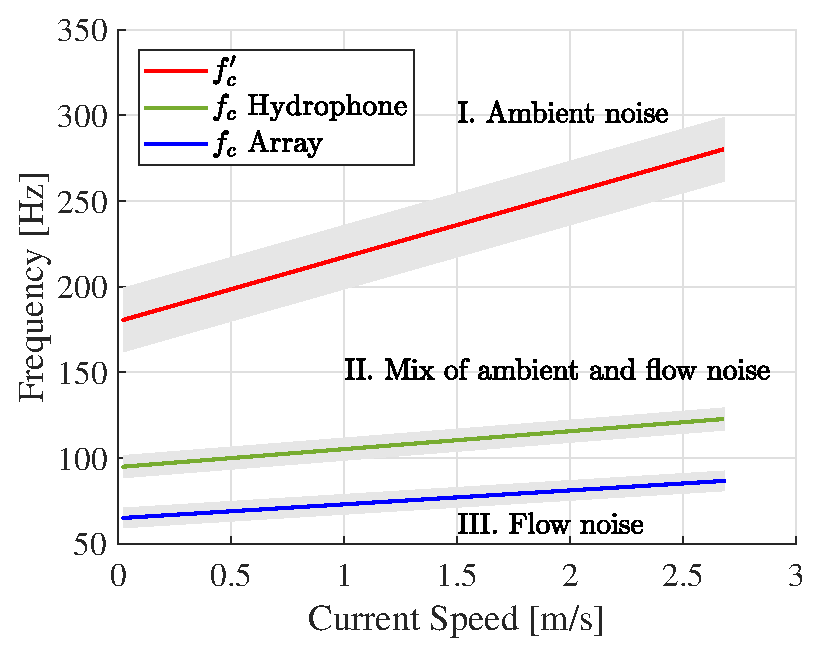
\includegraphics[width=0.7\textwidth]{figure7.eps}
	\end{center}
	\caption[Comparison of spectral sloping and spatial coherence thresholding]{
	\label{f:array_perform}
	Comparison of fixed single hydrophone spectral critical frequency (green), array spectral critical frequency (blue), and coherence critical frequency (red) as a function of current speed. Uncertainties are one standard deviation (shaded). Coherence critical frequency, $f^\prime_c$, separates region I, where flow noise is negligible, and region II, where flow and ambient noise are both present, while spectral critical frequency, $f_c$  separates regions II and III, where flow noise dominates. The coherent array effectively suppresses flow noise, as indicated by its lower boundary relative to the fixed single hydrophone. }
\end{figure}
\begin{figure}[!t]
	\begin{center}
		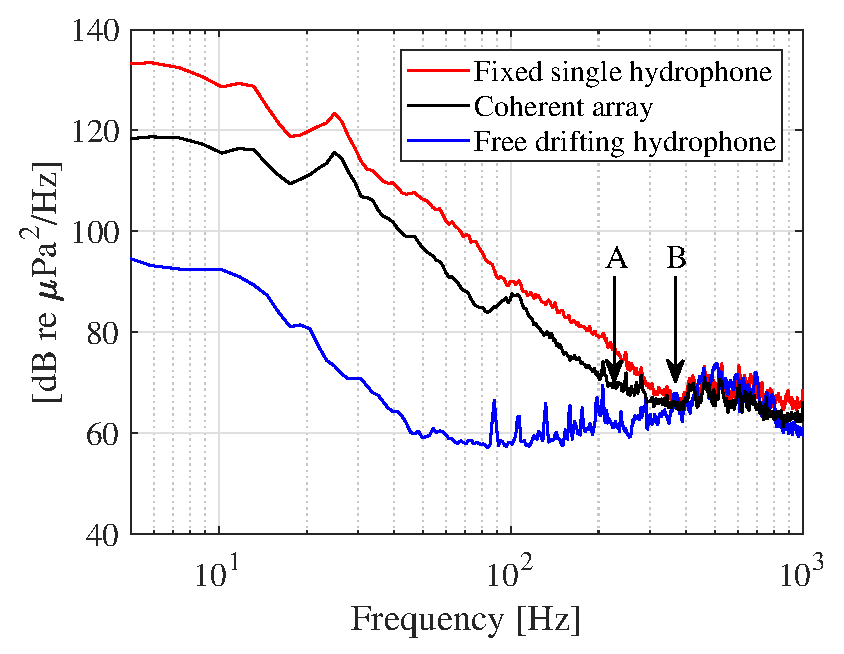
\includegraphics[width=0.7\textwidth]{figure8.eps} 
	\end{center}
	\caption[Comparison of hydrophone, coherent array, and guard buoy signals]{
	\label{f:comparison}
	Comparison of fixed single hydrophone (red), coherent array (black), and free drifting hydrophone (blue) signal power spectra at 1.5 hr into the deployment. The current speed at this moment was 2.2 m/s. A and B indicate the spectral critical frequencies of the coherent array and the fixed single hydrophone, respectively. The reduced levels and spectral critical frequency of the coherent array output relative to the fixed single hydrophone indicates flow noise suppression.  }
\end{figure}
The GuardBuoy spectrum behaves differently from the rest, exhibiting lower levels at frequencies below 100 Hz. A pronounced excursion in spectral slope is present at 10 Hz in the GuardBuoy spectrum, suggesting non-negligible flow noise is affecting the drifter's low-frequency measurements. This is typical of all moored or free drifting passive acoustic systems that have a surface expression or subsurface float. The fixed single hydrophone shows clear symptoms of flow noise at low frequencies. 

The spectra reveal that the coherent array spectra transitions to the ambient noise region at lower frequencies than the fixed single hydrophone. 
Furthermore, the coherent array signal levels are relatively lower than the fixed single hydrophone levels at all low frequencies, indicating moderate flow noise suppression. 
There is reasonable agreement between the GuardBuoy and coherent array above the critical frequency, with some difference above 700 Hz. This disparity is attributed to the lack of co-location between the array and the GuardBuoy, as they are vertically and horizontally displaced relative to each other.


%%%%%%%%%%%%%%%%%%%%%%%%%%%%%%%%%%%%%%%%%%%%%%%%%%%%%%%%%%%%%%%%%%%%
\section{Discussion}



\subsection{Spectral Critical Frequency}
Results show that critical frequency and flow speed are positively related, giving the intuitive result that flow noise is prevalent in fast current conditions. 
The spectral critical frequency presents a method of identifying flow noise prevalence within a signal. 

The spectral critical frequency marks where ambient noise and flow noise have equal power, and provides two important insights. Firstly, frequencies above the spectral critical frequency will contain a mixture of ambient noise and flow noise. Secondly, frequencies below the spectral critical frequency will be dominated by flow noise, since measurements in these frequencies contain spectral slopes that align with turbulence theory. These insights are important, as they provide useful context for future signal level and sound-source evaluations in tidal channel measurements. 



\subsection{Spatial Coherence}
Spatial coherence results for different sensor combinations show that there are two distinct coherence regions across the array: an incoherent flow noise region and a coherent ambient noise region. The prevalence of these regions is quantified with the coherence critical frequency. Moreover, the coherence critical frequency marks the frequency above which flow noise is absent. A least squared regression reveals that there is a positive relationship between flow speed and coherence critical frequency. 

The spectral critical frequency provides a lower boundary, below which ambient noise is negligible, and the coherence critical frequency provides an upper boundary, above which flow noise is negligible. Frequencies between these bounds contain a mixture of flow noise and ambient noise. This explains why the coherence critical frequencies are noticeably higher than those of the spectral method. The application of spectral and coherence critical frequencies provides insight on the relative extent of both ambient noise and flow noise within a signal. 



\subsection{Beamforming}
The linear array can be effectively treated as one sensor or hydrophone using broadside beamforming. This method generates signals that represent the coherent output of the entire array. These signals can be compared to a single fixed hydrophone using spectral analysis, as shown in Fig. \ref{f:array_perform}. The results of this analysis reveal relatively lower spectral critical frequencies for the array, suggesting that the coherent output from the array is less affected by flow noise and contains a greater extent of ambient noise. 

This interpretation is supported by a visual comparison of signals from the coherent array, a fixed single hydrophone, and the GuardBuoy (Fig. \ref{f:comparison}). The beamformed array contains lower levels at low frequencies and a lower spectral critical frequency than the fixed single hydrophone. The difference in signal levels between the coherent array and the fixed single hydrophone implies moderate flow noise suppression. Furthermore, the slight improvement in spectral critical frequency indicates that coherent averaging has enhanced the measurement of ambient noise. 
 
%By effectively treating the array as one sensor or hydrophone, signal processing can help address the pseudo-sound within low frequency data. 
%Coherent averaging shows promise as a method for suppressing flow noise and enhancing propagating ambient noise. 
%The coherent averaging employs a broadside approach with no steering angle, as outlined in \eqref{A}. 

 %A comparison of spectral critical frequencies shows that the coherent array contains relatively lower levels and critical frequencies than the fixed single hydrophone (Fig. \ref{f:array_perform}; Fig. \ref{f:comparison}). These results imply that the coherent array is comparatively less affected by flow noise and contains a greater extent of ambient noise.

It is important to note that the improvements in signal level and spectral critical frequency illustrated in Fig. \ref{f:array_perform} and Fig. \ref{f:comparison} are limited in magnitude. Further research would help determine the effectiveness of the coherent array as a method of flow noise suppression. This includes longer deployment periods, testing in different flow conditions, and experimentation in different bathymetric settings. Elimination of the mechanical noise floor would strengthen the present research. It would also be helpful to conduct tests with arrays of different length and a varied number of elements.
%%%%%%%%%%%%%%%%%%%%%%%%%%%%%%%%%%%%%%%%%%%%%%%%%%%%%%%%%%%%%%%%%%%%
\section{Conclusion}
Flow noise appears as: $f^{-5/3}$ noise when wavelength $>>$ sensor size, and $f^{-m}$ noise, where the sensor's finite dimension reduces the flow noise. The steepened slope, $f^{-m}$, is related to the flow speed over the array. The spectral critical frequency is used to identify where ambient noise is negligible and the coherence critical frequency is used to identify where flow noise is negligible. 

Coherent processing (beamforming) yields lower levels at low frequencies and a lower spectral critical frequency relative to a fixed single hydrophone. These improvements suggest that coherent processing could become an effective method of flow noise suppression. Experimentation in different flow settings and testing different array configurations would help determine the effectiveness of this approach. 


%%%%%%%%%%%%%%%%%%%%%%%%%%%%%%%%%%%%%%%%%%%%%%%%%%%%%%%%%%%%%%%%%%%%
\newpage



% if have a single appendix:
%\appendix[Proof of the Zonklar Equations]
% or
%\appendix  % for no appendix heading
% do not use \section anymore after \appendix, only \section*
% is possibly needed

% use appendices with more than one appendix
% then use \section to start each appendix
% you must declare a \section before using any
% \subsection or using \label (\appendices by itself
% starts a section numbered zero.)
%


%\appendices
%\section{Proof of the First Zonklar Equation}
%Appendix one text goes here.

% you can choose not to have a title for an appendix
% if you want by leaving the argument blank
%\section{}
%Appendix two text goes here.


% use section* for acknowledgment
%\section*{Acknowledgment}


%The authors would like to thank...


% Can use something like this to put references on a page
% by themselves when using endfloat and the captionsoff option.
\ifCLASSOPTIONcaptionsoff
  \newpage
\fi



% trigger a \newpage just before the given reference
% number - used to balance the columns on the last page
% adjust value as needed - may need to be readjusted if
% the document is modified later
%\IEEEtriggeratref{8}
% The "triggered" command can be changed if desired:
%\IEEEtriggercmd{\enlargethispage{-5in}}

% references section

% can use a bibliography generated by BibTeX as a .bbl file
% BibTeX documentation can be easily obtained at:
% http://mirror.ctan.org/biblio/bibtex/contrib/doc/
% The IEEEtran BibTeX style support page is at:
% http://www.michaelshell.org/tex/ieeetran/bibtex/
\bibliographystyle{IEEEtran}
% argument is your BibTeX string definitions and bibliography database(s)
\bibliography{IEEEabrv,literature}
%
% <OR> manually copy in the resultant .bbl file
% set second argument of \begin to the number of references
% (used to reserve space for the reference number labels box)
%\begin{thebibliography}{1}

%\bibitem{IEEEhowto:kopka}
%H.~Kopka and P.~W. Daly, \emph{A Guide to \LaTeX}, 3rd~ed.\hskip 1em plus
 % 0.5em minus 0.4em\relax Harlow, England: Addison-Wesley, 1999.

%\end{thebibliography}

% biography section
% 
% If you have an EPS/PDF photo (graphicx package needed) extra braces are
% needed around the contents of the optional argument to biography to prevent
% the LaTeX parser from getting confused when it sees the complicated
% \includegraphics command within an optional argument. (You could create
% your own custom macro containing the \includegraphics command to make things
% simpler here.)
%\begin{IEEEbiography}[{\includegraphics[width=1in,height=1.25in,clip,keepaspectratio]{mshell}}]{Michael Shell}
% or if you just want to reserve a space for a photo:

\begin{IEEEbiography}{Matthew Auvinen}
Biography text here.
\end{IEEEbiography}
% if you will not have a photo at all:
%\begin{IEEEbiography}[{\includegraphics[width=1in,height=1.25in,clip,keepaspectratio]{dave.eps}}]{David Barclay}
\begin{IEEEbiography}{David Barclay}
Biography text here.
\end{IEEEbiography}

% insert where needed to balance the two columns on the last page with
% biographies
%\newpage

%\begin{IEEEbiography}[{\includegraphics[width=1in,height=1.25in,clip,keepaspectratio]{dave.eps}}]{David Barclay}
%Biography text here.
%\end{IEEEbiography}

% You can push biographies down or up by placing
% a \vfill before or after them. The appropriate
% use of \vfill depends on what kind of text is
% on the last page and whether or not the columns
% are being equalized.

%\vfill

% Can be used to pull up biographies so that the bottom of the last one
% is flush with the other column.
%\enlargethispage{-5in}



% that's all folks




%\nocite{*}



% You must have at least 2 lines in the paragraph with the drop letter
% (should never be an issue)


%\hfill mds
 
%\hfill August 26, 2015

%\subsection{Subsection Heading Here}
%Subsection text here.

% needed in second column of first page if using \IEEEpubid
%\IEEEpubidadjcol

%\subsubsection{Subsubsection Heading Here}
%Subsubsection text here.


% An example of a floating figure using the graphicx package.
% Note that \label must occur AFTER (or within) \caption.
% For figures, \caption should occur after the \includegraphics.
% Note that IEEEtran v1.7 and later has special internal code that
% is designed to preserve the operation of \label within \caption
% even when the captionsoff option is in effect. However, because
% of issues like this, it may be the safest practice to put all your
% \label just after \caption rather than within \caption{}.
%
% Reminder: the "draftcls" or "draftclsnofoot", not "draft", class
% option should be used if it is desired that the figures are to be
% displayed while in draft mode.
%
%\begin{figure}[!t]
%\centering
%\includegraphics[width=2.5in]{myfigure}
% where an .eps filename suffix will be assumed under latex, 
% and a .pdf suffix will be assumed for pdflatex; or what has been declared
% via \DeclareGraphicsExtensions.
%\caption{Simulation results for the network.}
%\label{fig_sim}
%\end{figure}

% Note that the IEEE typically puts floats only at the top, even when this
% results in a large percentage of a column being occupied by floats.


% An example of a double column floating figure using two subfigures.
% (The subfig.sty package must be loaded for this to work.)
% The subfigure \label commands are set within each subfloat command,
% and the \label for the overall figure must come after \caption.
% \hfil is used as a separator to get equal spacing.
% Watch out that the combined width of all the subfigures on a 
% line do not exceed the text width or a line break will occur.
%
%\begin{figure*}[!t]
%\centering
%\subfloat[Case I]{\includegraphics[width=2.5in]{box}%
%\label{fig_first_case}}
%\hfil
%\subfloat[Case II]{\includegraphics[width=2.5in]{box}%
%\label{fig_second_case}}
%\caption{Simulation results for the network.}
%\label{fig_sim}
%\end{figure*}
%
% Note that often IEEE papers with subfigures do not employ subfigure
% captions (using the optional argument to \subfloat[]), but instead will
% reference/describe all of them (a), (b), etc., within the main caption.
% Be aware that for subfig.sty to generate the (a), (b), etc., subfigure
% labels, the optional argument to \subfloat must be present. If a
% subcaption is not desired, just leave its contents blank,
% e.g., \subfloat[].


% An example of a floating table. Note that, for IEEE style tables, the
% \caption command should come BEFORE the table and, given that table
% captions serve much like titles, are usually capitalized except for words
% such as a, an, and, as, at, but, by, for, in, nor, of, on, or, the, to
% and up, which are usually not capitalized unless they are the first or
% last word of the caption. Table text will default to \footnotesize as
% the IEEE normally uses this smaller font for tables.
% The \label must come after \caption as always.
%
%\begin{table}[!t]
%% increase table row spacing, adjust to taste
%\renewcommand{\arraystretch}{1.3}
% if using array.sty, it might be a good idea to tweak the value of
% \extrarowheight as needed to properly center the text within the cells
%\caption{An Example of a Table}
%\label{table_example}
%\centering
%% Some packages, such as MDW tools, offer better commands for making tables
%% than the plain LaTeX2e tabular which is used here.
%\begin{tabular}{|c||c|}
%\hline
%One & Two\\
%\hline
%Three & Four\\
%\hline
%\end{tabular}
%\end{table}


% Note that the IEEE does not put floats in the very first column
% - or typically anywhere on the first page for that matter. Also,
% in-text middle ("here") positioning is typically not used, but it
% is allowed and encouraged for Computer Society conferences (but
% not Computer Society journals). Most IEEE journals/conferences use
% top floats exclusively. 
% Note that, LaTeX2e, unlike IEEE journals/conferences, places
% footnotes above bottom floats. This can be corrected via the
% \fnbelowfloat command of the stfloats package.


\end{document}


